\documentclass{statsoc}
\usepackage{times}
%\documentstyle[nips07submit_09,times]{article}
\usepackage{fullpage}
\usepackage{color,graphicx}
\usepackage{eurosym}
\usepackage{amsmath}
\usepackage{amssymb}
\usepackage{verbatim}
\usepackage{mathrsfs}

\usepackage{footmisc}
\usepackage[utf8]{inputenc}
    

\usepackage{url}
\usepackage{algorithm}
\usepackage{algorithmicx}
\usepackage{algpseudocode}
\newtheorem{defn}{Definition}
    
% formatting tweaks
\newcommand{\te}{\!=\!} % thin equals
\newcommand{\tneq}{\!\neq\!}
\newcommand{\naive}{na\"{\i}ve}
\newcommand{\Naive}{Na\"{\i}ve}
\newcommand{\Levy}{L\'{e}vy}
\newcommand{\myvcenter}[1]{\ensuremath{\vcenter{\hbox{#1}}}} % vertical centering

% bold and caligraphic letters
\newcommand{\ba}{\mathbf{a}}
\newcommand{\bb}{\mathbf{b}}
\newcommand{\bc}{\mathbf{c}}
\newcommand{\bd}{\mathbf{d}}
\newcommand{\bg}{\mathbf{g}}
\newcommand{\bh}{\mathbf{h}}
\newcommand{\bs}{\mathbf{s}}
\newcommand{\bu}{\mathbf{u}}
\newcommand{\bw}{\mathbf{w}}
\newcommand{\bx}{\mathbf{x}}
\newcommand{\by}{\mathbf{y}}
\newcommand{\hyp}{{\mathcal H}}
\newcommand{\model}{{\mathcal M}}
\newcommand{\data}{{\mathcal D}}
\newcommand{\Z}{{\mathcal Z}}
\newcommand{\N}{{\mathcal N}}
\newcommand{\M}{{\mathcal M}}
\newcommand{\F}{{\mathcal F}}
\newcommand{\vS}{{\vec{S}}}
\newcommand{\cS}{{\mathcal S}}
\newcommand{\vcS}{{\vec{\mathcal S}}}
\newcommand{\cT}{{\mathcal T}}
\newcommand{\cN}{{\mathcal N}}
\newcommand{\ocS}{\overline{\mathcal S}}
\newcommand{\Tu}{\mathcal{T}^{\cup}}
\newcommand{\Su}{\mathcal{S}^{\cup}}
\newcommand{\vSu}{\vec{\mathcal{S}}^{\cup}}
\newcommand{\Mu}{\mathcal{M}^{\cup}}
\newcommand{\muu}{\mu^{\cup}}
\newcommand{\vmuu}{\vec{\mu}^{\cup}}
\newcommand{\mul}{\mu^{<}}
\newcommand{\tmuu}{\tilde{\mu}^{\cup}}
\newcommand{\oSigma}{\overline{\Sigma}}
\newcommand{\vSigma}{\vec{\Sigma}}
\newcommand{\dif}{\mathrm{d}}

% arrows without lots of space
\newcommand{\la}{\!\leftarrow\!}
\newcommand{\ra}{\!\rightarrow\!}
\newcommand{\lra}{\!\leftrightarrow\!}

% Miscellaneous mathematics
\newcommand{\nth}{^{\left( n \right)}}
\newcommand{\mth}{^{\left( m \right)}}
\newcommand{\nnth}[1]{^{\left(#1\right)}}
\DeclareMathOperator*{\argmax}{argmax}
\DeclareMathOperator*{\argmin}{argmin}
\newcommand{\pdd}[2]{\frac{\partial #1}{\partial #2}}

% Colors
%\usepackage{color}
\definecolor{mypine}{rgb}{0.05,0.45,0.05}
\definecolor{mydarkred}{rgb}{0.75,0.05,0.05}
\definecolor{mypurple}{rgb}{0.75,0.0,0.75}
\definecolor{mygray}{rgb}{0.35,0.35,0.35}
\definecolor{mylightgray}{rgb}{0.5,0.5,0.5}
\newcommand{\Red}{\textcolor{red}}
%\newcommand{\Red}{\textcolor{mydarkred}}
\newcommand{\Blue}{\textcolor{blue}}
\newcommand{\Gray}{\textcolor{mygray}}
\newcommand{\LightGray}{\textcolor{mylightgray}}
\newcommand{\Purple}{\textcolor{mypurple}}
\newcommand{\Green}{\textcolor{mypine}}
\newcommand{\Cyan}{\textcolor{cyan}}
\newcommand{\PineGreen}{\textcolor{mypine}}
\newcommand{\DarkGreen}{\textcolor{mypine}}

\newcommand{\txss}{\textsuperscript}

% defined again below
%\def\l({\left(}
%\def\r){\right)}



\DeclareMathOperator*{\KL}{KL}

\def\bS{\mathbf{S}}
\def\tbS{\tilde{\bS}}
\def\tS{\tilde{S}}
\def\ts{\tilde{s}}
\def\tt{\tilde{t}}
\def\tT{\tilde{T}}
\def\tA{\tilde{A}}
\def\tI{\tilde{I}}
\def\tP{\tilde{P}}
\def\tR{\tilde{R}}
\def\tW{\tilde{W}}
\def\tw{\tilde{w}}
\def\tF{\tilde{F}}
\def\tG{\tilde{G}}
\def\tE{\tilde{E}}
\def\bL{\mathbf{L}}

\def\ind{1}

\newcommand{\avg}[1]{\langle{#1} \rangle}

\def\naive{na\"{\i}ve}
\def\hlambda{\hat{\lambda}}
\def\ulmb{\underline{\lambda}}
\def\olmb{\overline{\lambda}}
\def\uR{\underline{R}}
\def\oR{\overline{R}}
\def\Reps{R^{\epsilon}}
\def\leps{\lambda^{\epsilon}}

% these break default latex commands for, e.g., Swedish names
%\def\l({\left(} 
%\def\r){\right)}

\def\matern{Mat\'{e}rn }

\newcommand{\NOTE}[1]{\textcolor{red}{[#1]}}
\newcommand{\given}{\,|\,}

%\newtheorem{defn}{Definition} 
\newtheorem{prop}[defn]{Proposition} 
\newtheorem{thrm}[defn]{Theorem} 
\newtheorem{coro}[defn]{Corollary}
\newcommand{\vinayak}[1]{\textcolor{red}{[Vinayak: #1]}}

\newcounter{subfigure}

\title{Bayesian inference for \matern repulsive processes (Supplementary material)}
\author{Vinayak Rao\thanks{Corresponding author}}
\address{Department of Statistics, Purdue University, USA}
\author{Ryan P. Adams}
\address{School of Engineering and Applied Sciences, Harvard University, USA}
\author{David Dunson}
\address{Department of Statistical Science, Duke University, USA}
\date{}

% Vinayak: to do: David section 6

\begin{document}

\maketitle

\section{Supplementary}

  \begin{figure}
  \begin{minipage}[h]{0.22\linewidth}
  \caption[Post Pred]{Posterior predictive values of J-functions for the Swedish pine tree dataset. (Top left) is the \matern hardcore model,
  (top right) is the softcore model, and (bottom left) is probabilistic thinning. (Bottom right): predictive values for a Strauss process fit.}
  \label{fig:swed_J_pred}
  \end{minipage}
  \begin{minipage}[h]{0.76\linewidth}
  \begin{minipage}[h]{0.49\linewidth}
  \centering
  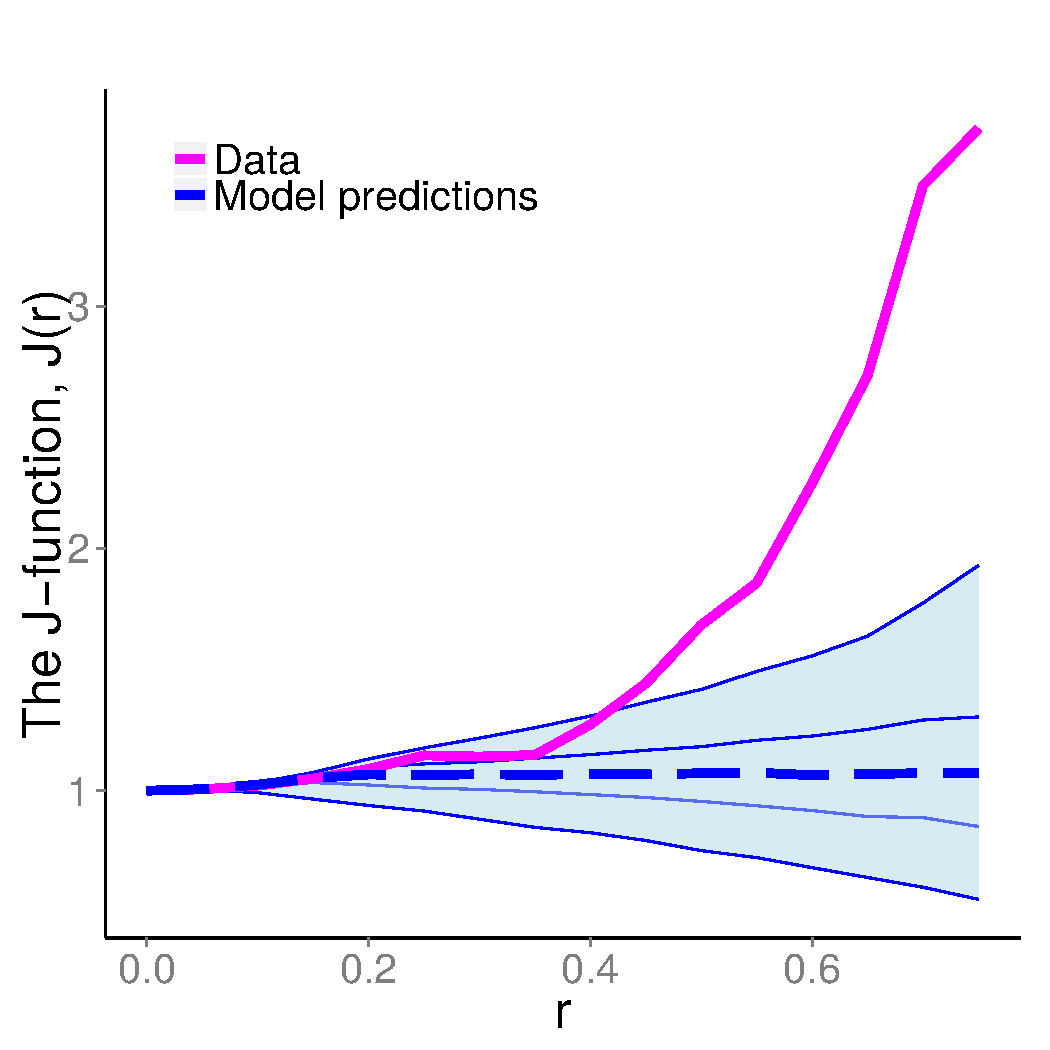
\includegraphics[width=0.99\textwidth]{figs/Jfunc_postpred_R10/swed_hc.pdf}
  \end{minipage}
  \begin{minipage}[h]{0.49\linewidth}
  \centering
  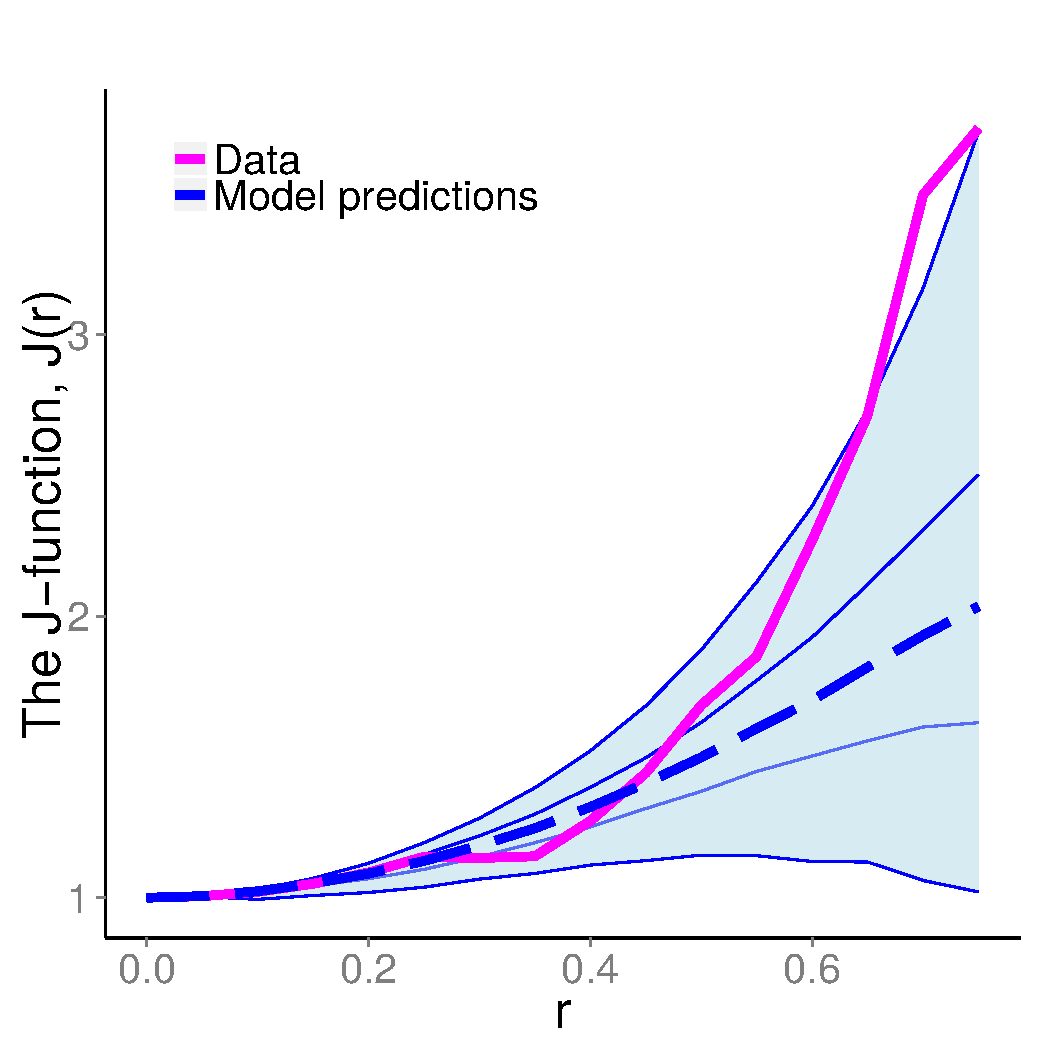
\includegraphics[width=0.99\textwidth]{figs/Jfunc_postpred_R10/swed_sc.pdf}
  \end{minipage}
  \begin{minipage}[h]{0.49\linewidth}
  \centering
  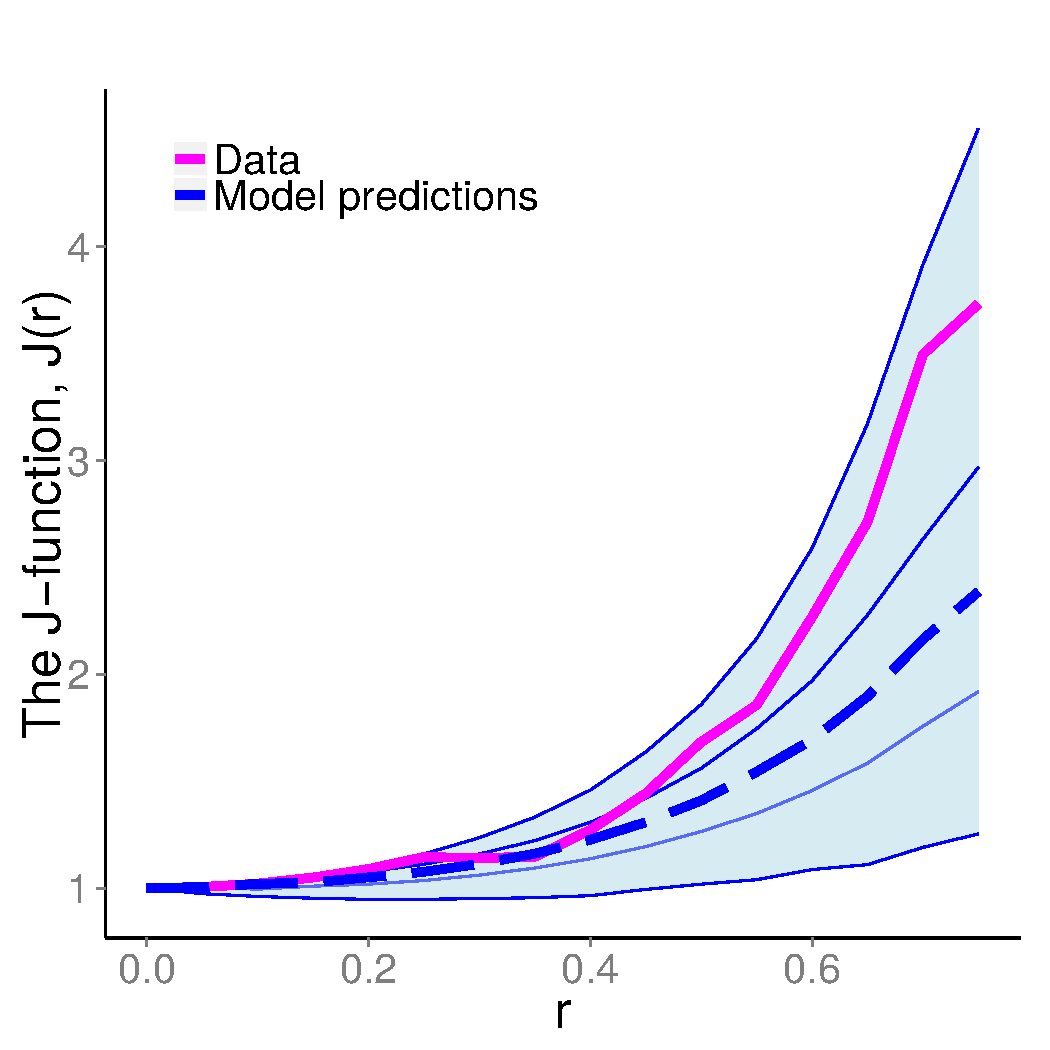
\includegraphics[width=0.99\textwidth]{figs/Jfunc_postpred_R10/swed_prob_full.pdf}
  \end{minipage}
  \begin{minipage}[h]{0.49\linewidth}
  \centering
  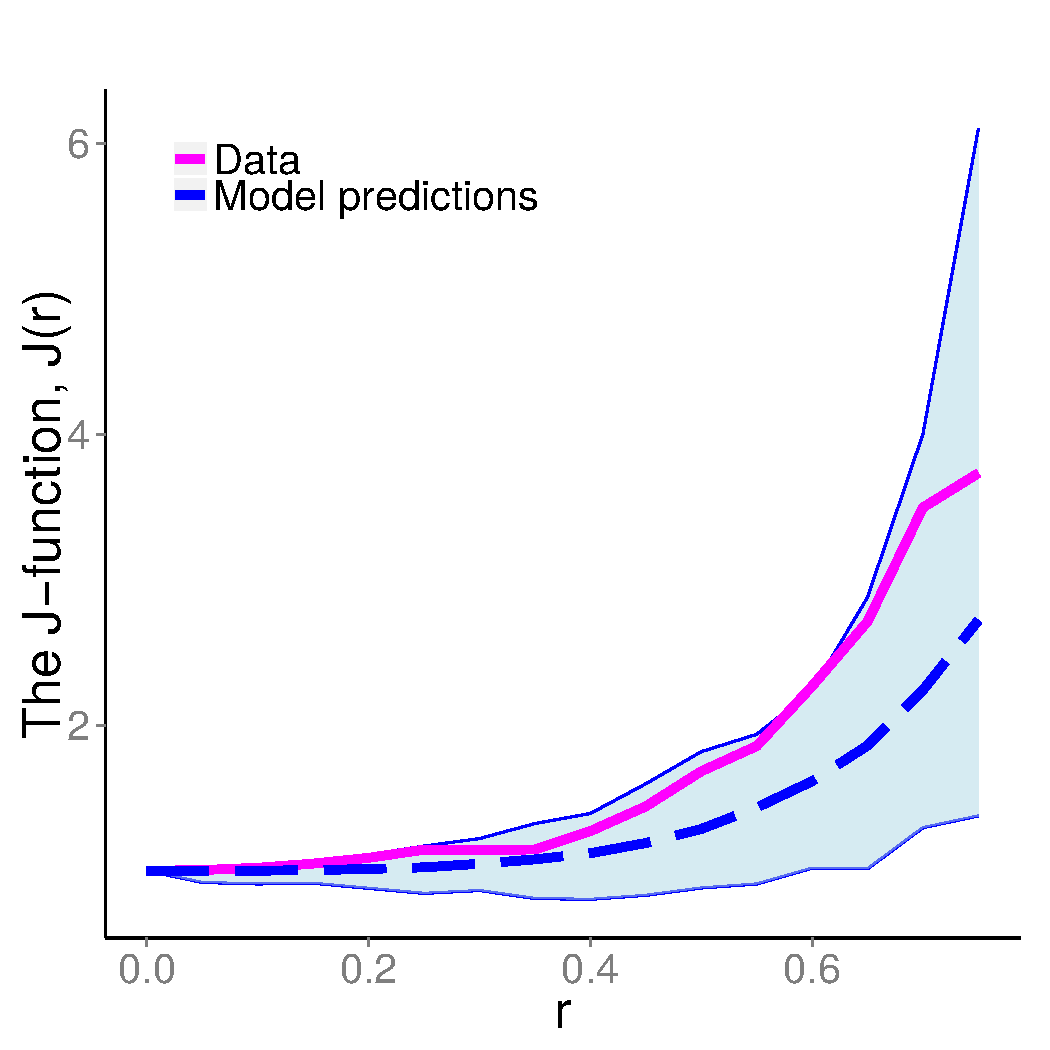
\includegraphics[width=0.98\textwidth]{figs/Jfunc_postpred_R10/swed_gibbs.pdf}
  \end{minipage}
  \end{minipage}
  \end{figure}

  The plots  of figure \ref{fig:swed_J_pred} consider the J-function (van Lieshout and Baddeley, 1996), a measure of spatial interaction with 
$J(r)$ corresponding to the ratio of the 
  probability there is no event at distance $r$ from another event to the probability there is no event at distance $r$ from an arbitrary point
  in the space. For a Poisson process, these two probabilities are equal, so that $J(r)$ equals $1$. Repulsion correspond to
  $J(r) > 1$, while $J(r)<1$ suggests a clustered pattern. 
  The continuous magenta line in figure~\ref{fig:swed_J_pred} plots the empirical $J(r)$ as a function of distance $r$ for the 
  pine tree dataset. Again we see that this is a non-Poisson repulsive process. The blue envelope shows posterior predictive estimates for the J-function 
  produced by fitting the \matern type-III hardcore process (top left), softcore process (top right) and with probabilistic thinning (bottom left). 
  See the main text for a description of these. 
  As with the L-function, the predictive intervals for the hardcore and softcore processes do not fit the data, but contrast the generalized \matern
with probabilistic thinning does a much better job. The bottom right subplot shows predictions from a MLE fit of a Strauss process, which also
produces reasonable (but not good)  fits.

  \begin{figure}
  \begin{minipage}[h]{0.24\linewidth}
  \caption[Post Pred]{(Top row): Posterior predictive values of the J-functions for the \matern model with probabilistic thinning for mild (left) and 
  moderate (right) neuropathy. (Bottom row): Corresponding predictive values for Strauss process fits.}
%  \caption[Post Pred]{Posterior predictive values of J-functions for the Swedish pine tree dataset. (Top left) is the \matern hardcore model,
%  (top right) is the softcore model, and (bottom left) is probabilistic thinning. (Bottom right) is the fit for a Strauss process.}
  \label{fig:diab_Jfunc}
  \end{minipage}
  \centering
  \begin{minipage}[h]{0.74\linewidth}
  \begin{minipage}[h]{0.49\linewidth}
  \centering
  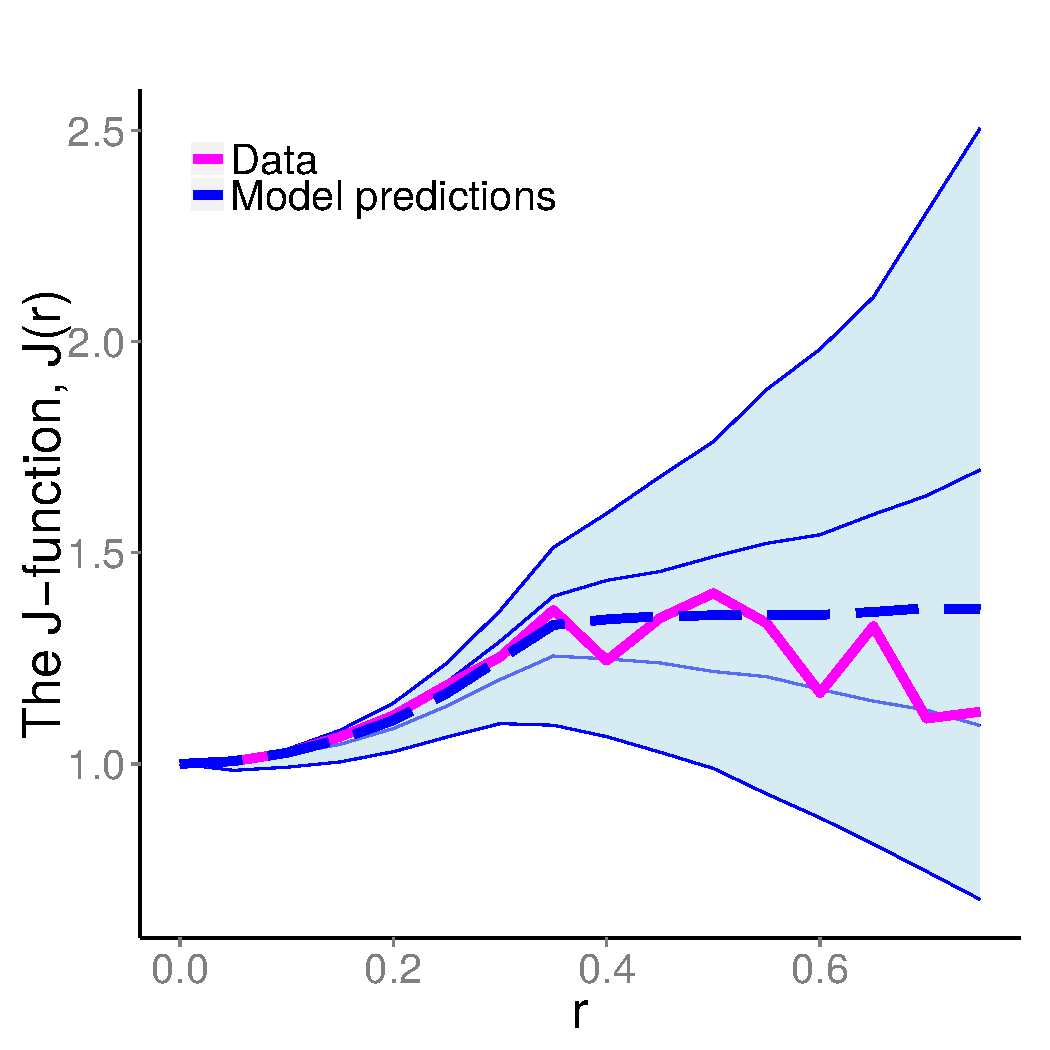
\includegraphics[width=0.98\textwidth]{figs/Jfunc_postpred_R10/mild1_prob_full.pdf}
  \end{minipage}
  \begin{minipage}[h]{0.49\linewidth}
  \centering
  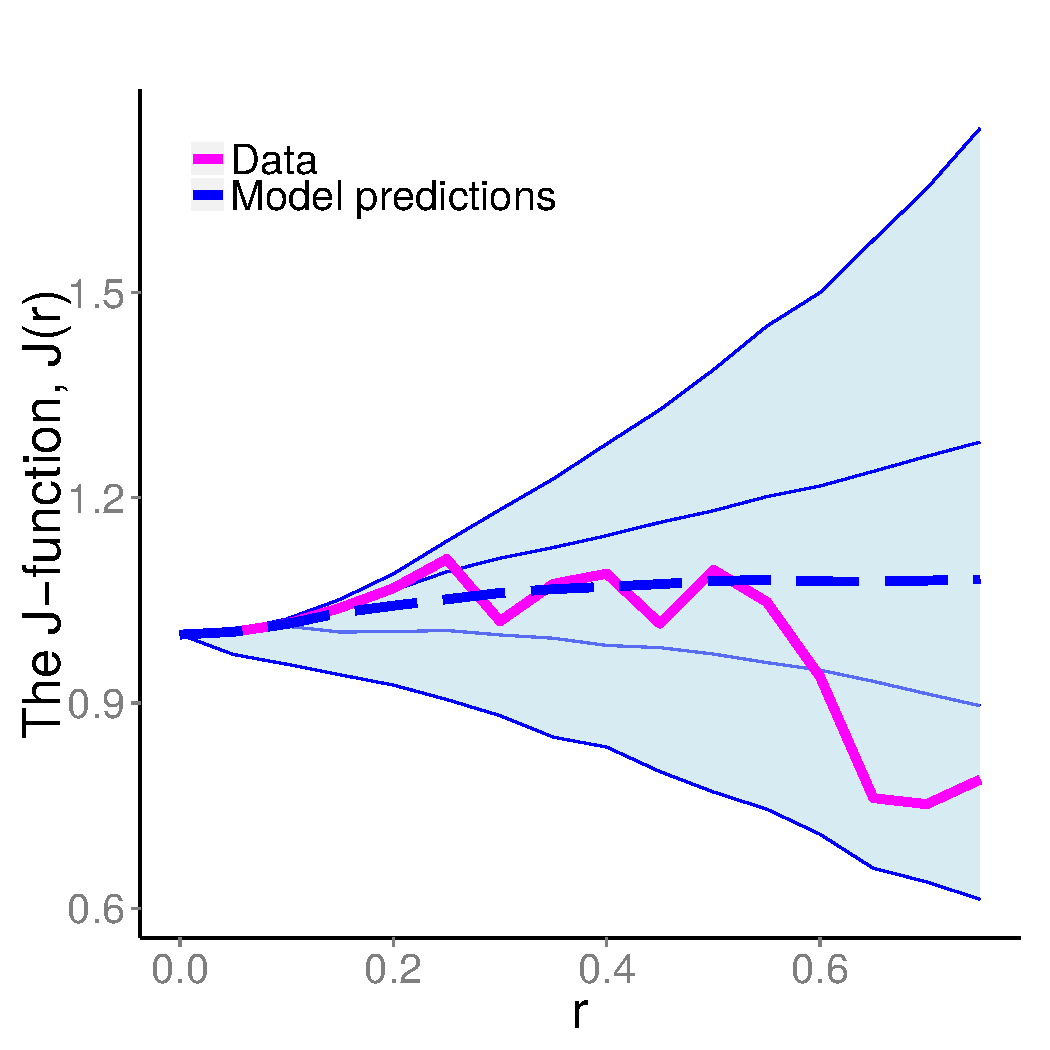
\includegraphics[width=0.98\textwidth]{figs/Jfunc_postpred_R10/mod1_prob_full.pdf}
  \end{minipage}
  \begin{minipage}[h]{0.49\linewidth}
  \centering
  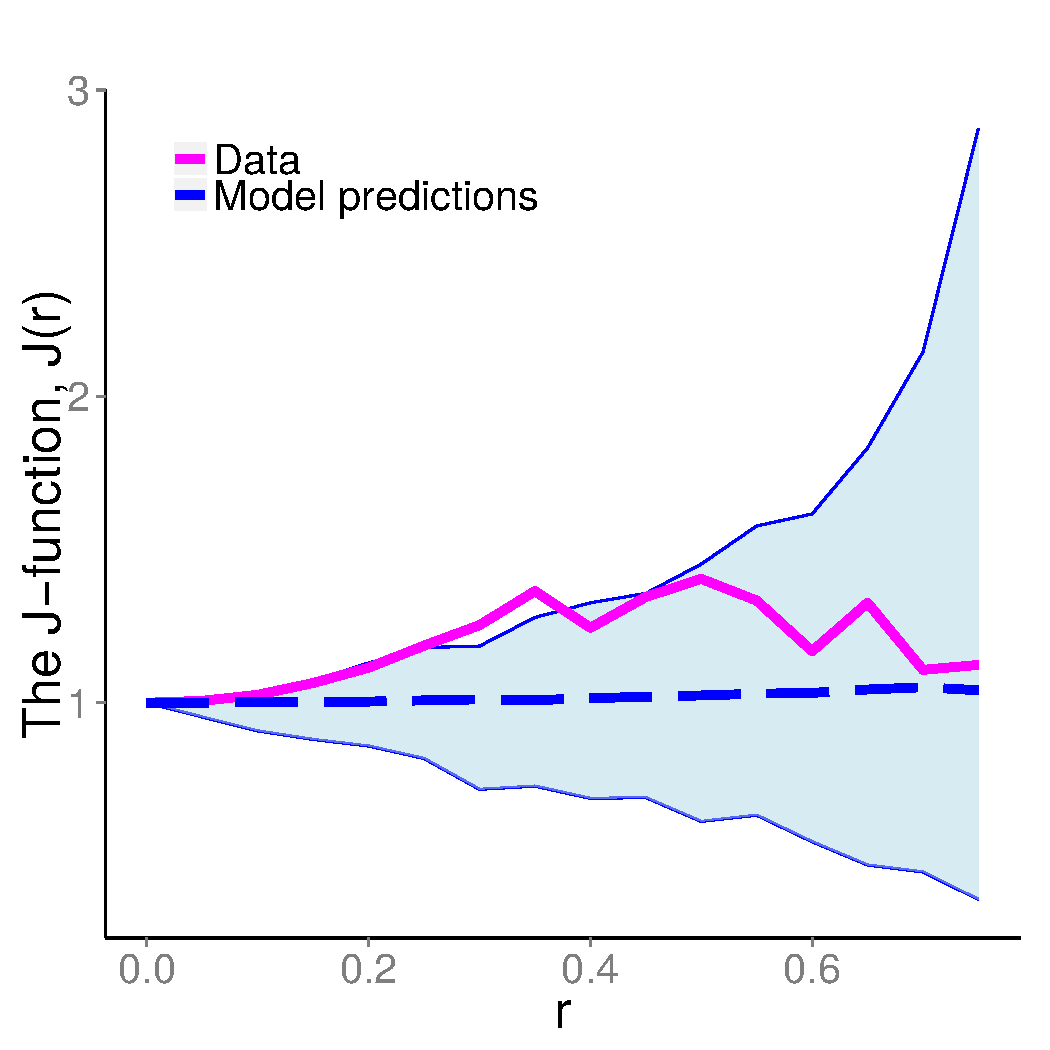
\includegraphics[width=0.98\textwidth]{figs/Jfunc_postpred_R10/mild1_gibbs.pdf}
  \end{minipage}
  \begin{minipage}[h]{0.49\linewidth}
  \centering
  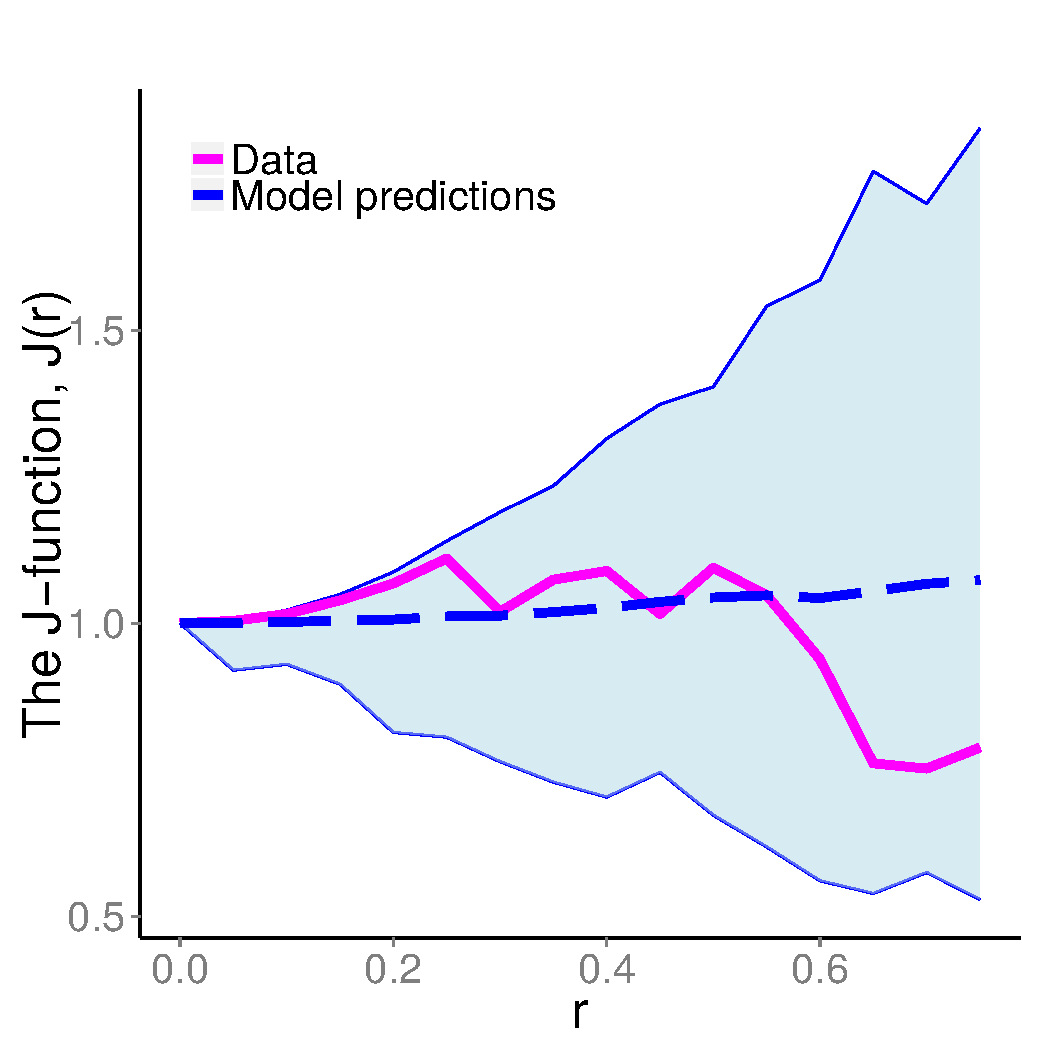
\includegraphics[width=0.98\textwidth]{figs/Jfunc_postpred_R10/mod1_gibbs.pdf}
  \end{minipage}
  \end{minipage}
  \end{figure}
The top row of figure \ref{fig:diab_Jfunc} shows posterior predictive values for a \matern process with probabilistic thinning for
mild (left) and moderate (right) neuropathy. The bottom row shows fits for a Strauss process, again, these are worse.
  \begin{figure}
  \centering
  \begin{minipage}[h]{0.28\linewidth}
  \caption{Inhomogeneous J-function for the Greyhound dataset: (left) posterior predictive values for nonstationary \matern, and (right)
  fit of an inhomogeneous Poisson process} 
  \label{fig:grey_ncscga_jfunc}
  \end{minipage}
  \begin{minipage}[h]{0.32\linewidth}
    \centering
    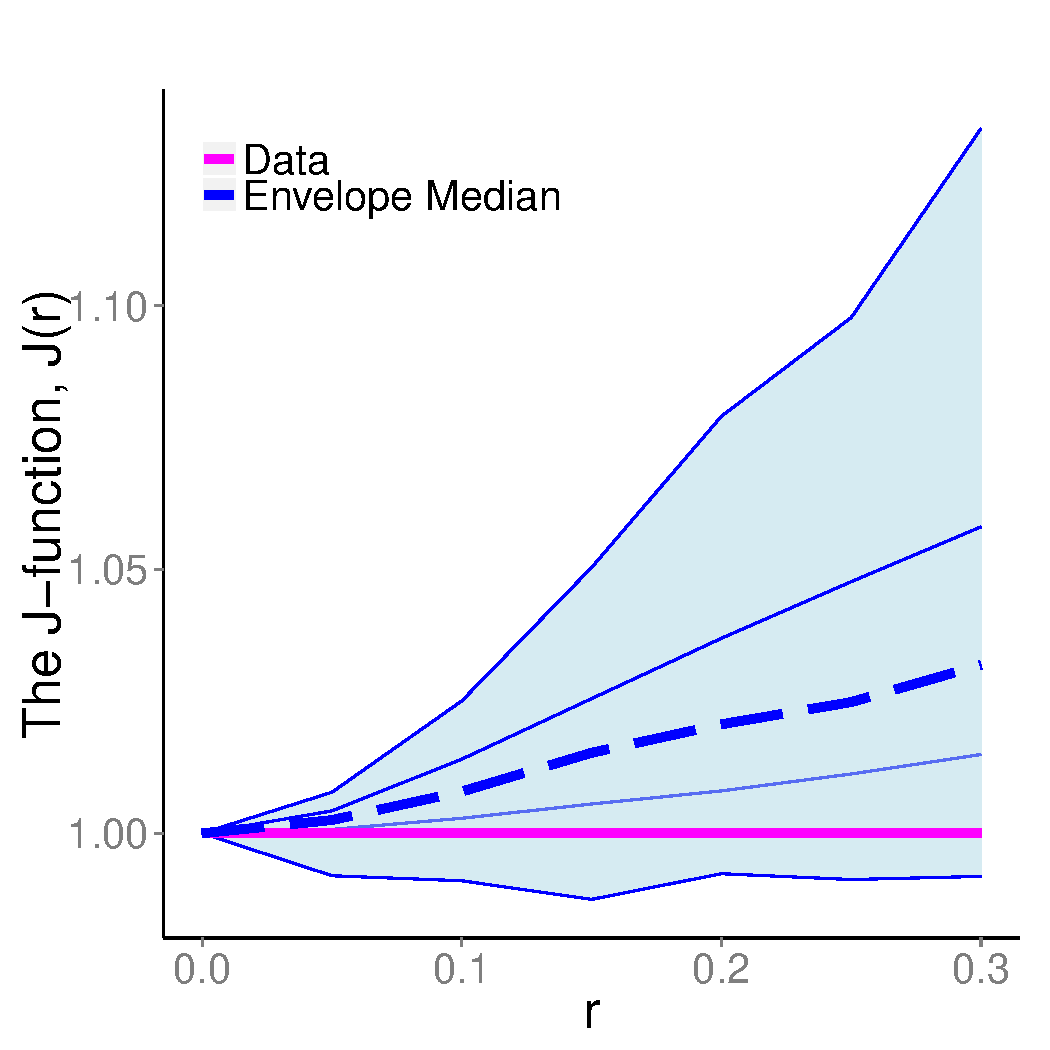
\includegraphics[width=0.98\textwidth, angle=0]{figs/greyhound_NCSCGA_matern_J.pdf}
  \end{minipage}
  \begin{minipage}[h]{0.32\linewidth}
  \centering
    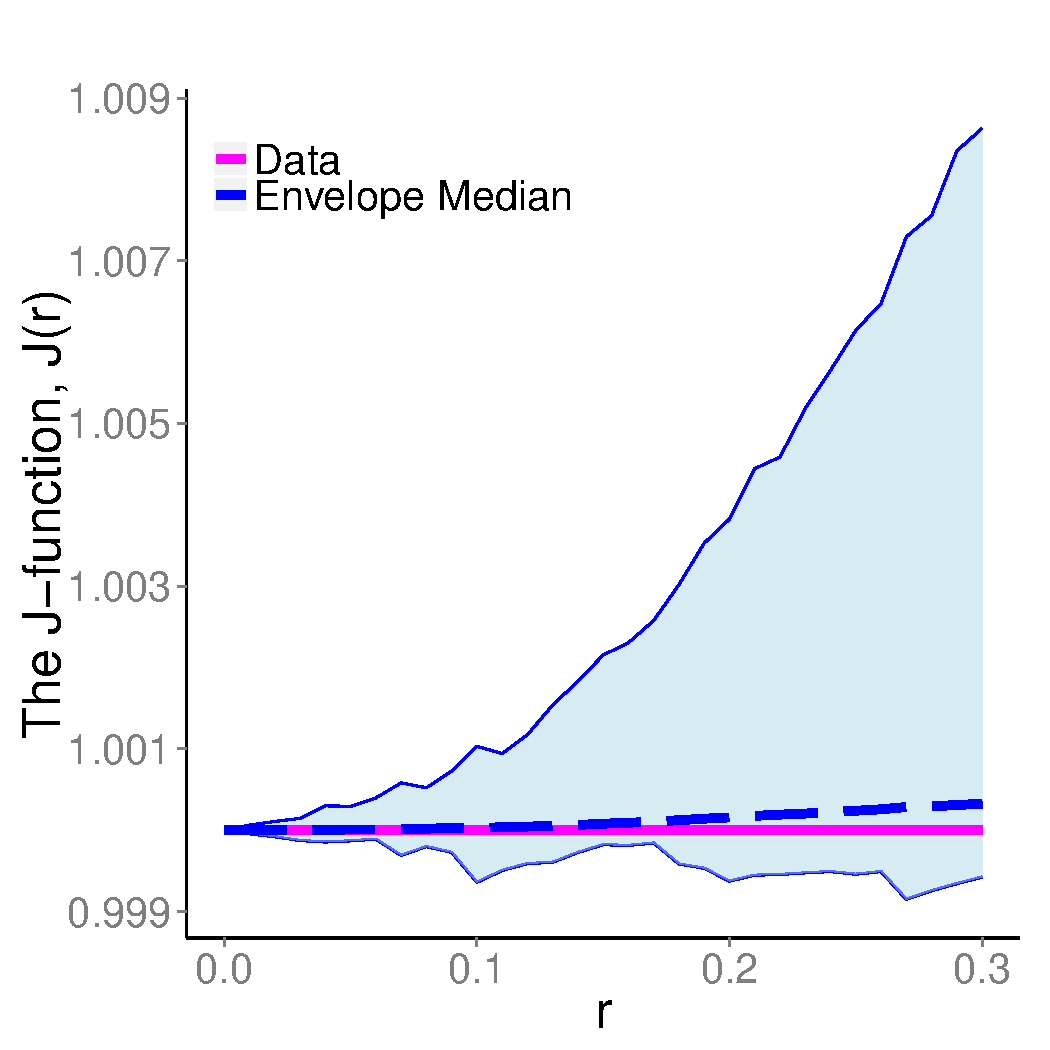
\includegraphics[width=0.98\textwidth, angle=0]{figs/greyhound_NCSCGA_poisson_J.pdf}
  \end{minipage}
  \end{figure}

Figure \ref{fig:grey_ncscga_jfunc} shows the nonstationary J-function estimated from the Greyhound dataset. This statistic does not capture
a significant deviation from Poisson (unlike the L-function), but both the inhomogeneous \matern model and the inhomogeneous Poisson process
fit it well.


\end{document}
